\section{Resultados e Discussão}
\label{sec:resultados}

A aplicação do pipeline computacional aos registros licitatórios do exercício de 2025 do município de Divinópolis/MG permitiu reconstruir a rede de participação, co-disputa e relações societárias e selecionar, de forma determinística, pares de empresas com sobreposições cadastrais ou societárias relevantes. Esses resultados são tratados como sinais de risco para triagem, e não como comprovação de simulação de competitividade ou de ilícito.

\subsection{Caracterização Topológica da Rede Completa}

Após a consolidação das tabelas do SICOM/TCE-MG e o enriquecimento societário junto à base da Receita Federal (BrasilAPI), construiu-se o grafo heterogêneo multicamada composto por três partições de vértices: órgãos públicos, empresas licitantes e respectivos sócios ou controladores, como mostrado na Fig.~\ref{fig:grafo-completo}.  A projeção visual da rede completa evidencia o fenômeno de ofuscamento estrutural (\emph{hairball effect}) inerente a grandes redes de compras públicas. A
distribuição dessas entidades é apresentada na Tabela~\ref{tab:vertices}.
\begin{table}[!h]
  \centering
  \caption{Distribuição dos Vértices por Categoria}
  \label{tab:vertices}
  \footnotesize
  \begin{tabular}{lrr}
    \hline
    \textbf{Categoria} & \textbf{Quantidade} & \textbf{Descrição} \\
    \hline
    Órgãos públicos & 2 & 2 órgãos municipais \\
    Empresas licitantes & 674 & 673 PJ e 1 PF \\
    Sócios e controladores & 1.112 & 1.044 PF e 68 PJ \\
    \hline
    \textbf{Total} & \textbf{1.788} & \\
    \hline
  \end{tabular}
\end{table}

Na partição dos órgãos públicos, a Prefeitura Municipal (\texttt{Orgao\_02}) concentra 245 licitações, enquanto a
Câmara Municipal (\texttt{Orgao\_01}) participa de 19
licitações. Essa distribuição evidencia a predominância
da atividade contratante do Poder Executivo na rede analisada. 
As relações entre os vértices são representadas por quatro
camadas de arestas, cujas respectivas quantidades e características são apresentadas na Tabela~\ref{tab:arestas}.

\begin{table}[!h]
  \centering
  \caption{Distribuição das Arestas por Camada Relacional}
  \label{tab:arestas}
  \resizebox{\columnwidth}{!}{%
    \begin{tabular}{@{}lrl@{}}
      \toprule
      \textbf{Camada} & \textbf{Quantidade} & \textbf{Relação Representada} \\
      \midrule
      \texttt{Participou\_Licitacao} & 680   & Participação em licitações \\
      \texttt{Concorreu\_Contra}     & 4.059 & Concorrência entre empresas \\
      \texttt{É\_Dono\_De}           & 1.132 & Propriedade societária \\
      \texttt{Vinculo\_Suspeito}     & 43    & Vínculos acima do limiar de risco \\
      \midrule
      \textbf{Total}                 & \textbf{5.914} & \\
      \bottomrule
    \end{tabular}%
  }
\end{table}

A camada \texttt{Participou\_Licitacao} estabelece as
relações entre fornecedores e órgãos contratantes,
enquanto \texttt{Concorreu\_Contra} representa as disputas comerciais entre pares de empresas. A camada
\texttt{É\_Dono\_De} modela os vínculos de propriedade
entre sócios e empresas. Por fim, a camada
\texttt{Vinculo\_Suspeito} reúne as relações identificadas
pelo modelo de pontuação multidimensional, retidas
a partir do limiar mínimo $s(a,b) \geq 1{,}00$. Assim, as 43 arestas dessa camada correspondem aos 37 pares de risco médio e aos seis pares de risco alto.

\begin{figure}[!t]
  \centering
  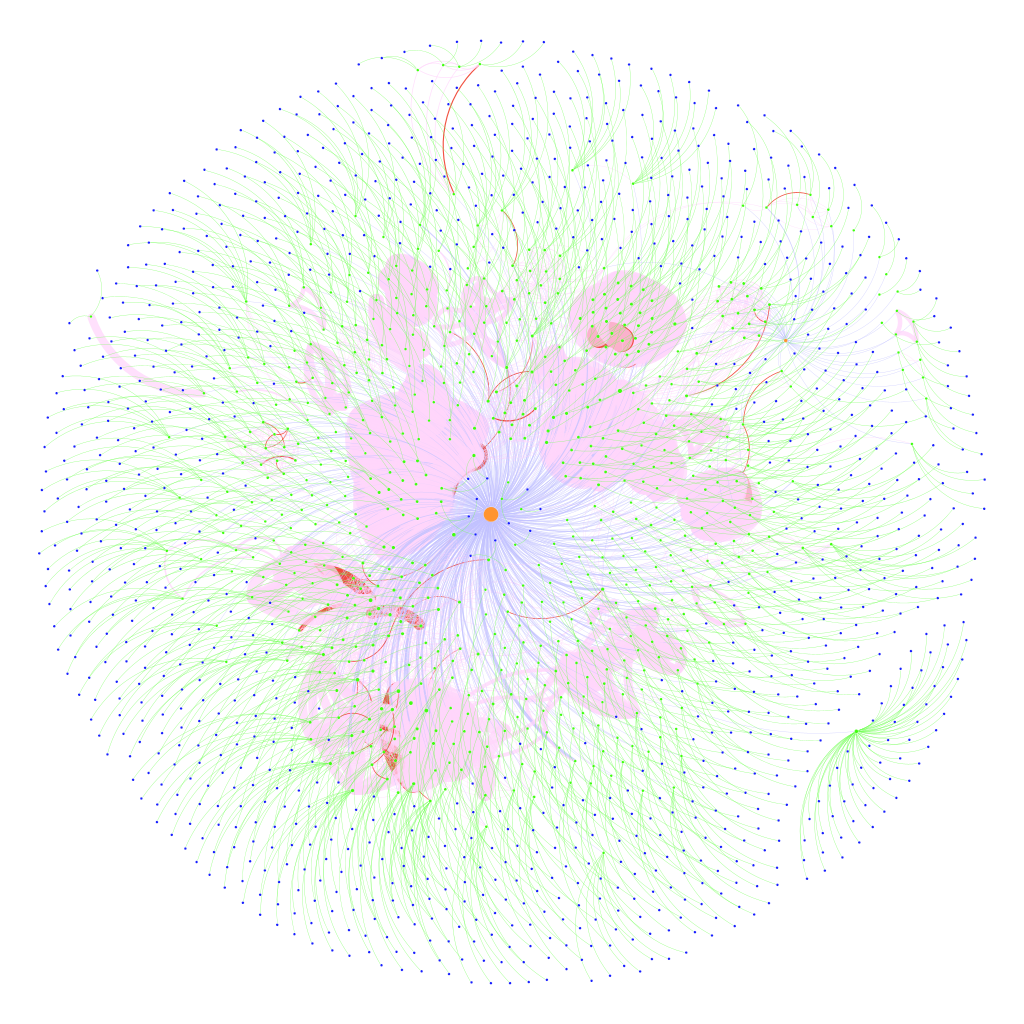
\includegraphics[width=\linewidth]{figures/grafo_completo}
  \caption{Topologia completa da rede heterogênea multicamada de contratações públicas de Divinópolis/MG em 2025 ($|V| = 1.788$, $|E| = 5.914$). O vértice central em laranja (\texttt{Orgao\_02} — Prefeitura Municipal) exerce forte atração gravitacional sobre as empresas licitantes (vértices verdes) por meio das arestas azuis claras (\texttt{Participou\_Licitacao}), enquanto o agrupamento isolado no quadrante inferior direito representa o polo periférico do Legislativo (\texttt{Orgao\_01} — Câmara Municipal). As nuvens densas em rosa claro (\texttt{Concorreu\_Contra}) e o halo externo de sócios em azul (\textit{Sócio Real}, ligados por arestas verdes \texttt{É\_Dono\_De}) obscurecem as 43 arestas vermelhas (\texttt{Vinculo\_Suspeito}).}
  \label{fig:grafo-completo}
\end{figure}

\subsection{Estratificação do Escore Multidimensional e Eficiência da Redução Algorítmica}

A avaliação cadastral, societária e onomástica dos 4.059 pares de empresas concorrentes identificou 202 pares com sobreposição
positiva, caracterizada por $s(a,b)>0$. A estratificação desses pares em faixas de criticidade permitiu distinguir coincidências
onomásticas de baixa relevância de relações com maior potencial indiciário, conforme apresentado na Tabela~\ref{tab:estratificacao}.
\begin{table}[!h]
  \centering
  \caption{Estratificação dos Pares Concorrentes por Faixa de Risco}
  \label{tab:estratificacao}
  \footnotesize
  \begin{tabular}{lrrp{3.2cm}}
    \hline
    \textbf{Faixa} & \textbf{Pares} & \textbf{Intervalo} & \textbf{Critério de Classificação} \\
    \hline
    Baixo & 159 & $0 < s < 1{,}00$ & Coincidências isoladas de sobrenomes triviais \\
    Médio & 37  & $1{,}00 \leq s < 2{,}00$ & Sobreposições onomásticas sem identidade cadastral direta \\
    Alto  & 6   & $s \geq 2{,}00$ & Identidade cadastral ou societária direta e/ou escore elevado \\
    \hline
    \textbf{Total} & \textbf{202} & & \\
    \hline
  \end{tabular}
\end{table}

Os 159 pares classificados como de baixo risco correspondem predominantemente a coincidências isoladas de sobrenomes
triviais, às quais foi atribuído peso de 0{,}25. Por esse motivo, esses pares foram excluídos da camada indiciária. Os 37 pares
de risco médio, associados a sobreposições onomásticas de menor frequência ou segundos prenomes, sem correspondência direta de
sócios, endereços ou telefones, foram mantidos no grafo completo como relações de monitoramento. Por sua vez, os seis pares de
alto risco foram selecionados como alvos prioritários para investigação, em razão dos escores elevados ou da presença de
identidades cadastrais e societárias diretas.

Após a estratificação, a cadeia de redução topológica, implementada no módulo \texttt{reduzir\_grafo.py}, foi aplicada
sequencialmente ao grafo completo. O procedimento reduziu a estrutura de 1.788 para 26 vértices e de 5.914 para 23 arestas,
correspondendo a uma redução de 98{,}55\% e 99{,}61\%, respectivamente. A evolução das métricas estruturais em cada
etapa do processamento é apresentada na Tabela~\ref{tab:reducao_topologica}.

\begin{table}[!h]
  \centering
  \caption{Evolução Métrica do Pipeline de Redução Topológica}
  \label{tab:reducao_topologica}
  \resizebox{\columnwidth}{!}{%
    \begin{tabular}{@{}p{2.6cm}rrp{4.2cm}@{}}
      \toprule
      \textbf{Etapa do Pipeline} & \textbf{Vértices} & \textbf{Arestas} & \textbf{Resultado Estrutural} \\
      \midrule
      Grafo completo & 1.788 & 5.914 & Representação integral da rede multicamada, composta por quatro camadas relacionais. \\
      1. Subgrafo filtrado por arestas ($\theta \geq 2{,}00$) & 1.788 & 23 & Retenção de seis relações \texttt{Vinculo\_Suspeito} e 17 relações \texttt{É\_Dono\_De}. \\
      2. Poda de vértices isolados & 26 & 23 & Remoção de 1.762 vértices de grau zero. \\
      3. Componentes conexas (\textit{Union-Find}) & 26 & 23 & Identificação de seis componentes conexas independentes, contendo 12 empresas e 14 sócios. \\
      4. Enumeração de triângulos ($K_3$) & -- & -- & Identificação de três motivos $K_3$, distribuídos em dois componentes conexos. \\
      \bottomrule
    \end{tabular}%
  }
\end{table}

A redução estrutural evidencia a capacidade do procedimento algorítmico de concentrar a análise nas relações de maior criticidade. Inicialmente, a aplicação do limiar $\theta \geq 2{,}00$ preservou 23 arestas, correspondentes a seis vínculos suspeitos e 17 relações societárias associadas. Em seguida, a remoção dos vértices sem incidência de arestas reduziu a rede a 26 vértices, mantendo integralmente as
relações selecionadas.

Na etapa seguinte, a aplicação do algoritmo \textit{Union-Find} permitiu identificar seis componentes conexas independentes, delimitando os núcleos relacionais para análise individualizada. Por fim, a enumeração de triângulos identificou três motivos estruturais $K_3$, concentrados em dois dos seis componentes. Esses motivos foram utilizados para identificar estruturas de controle societário compartilhado entre empresas concorrentes, cuja análise detalhada é apresentada na Subseção~\ref{subsec:nucleos_alto_risco}.



A análise quantitativa apresentada nesta seção concentra-se nas relações licitatórias, societárias e cadastrais. Embora o fluxo metodológico contemple uma etapa complementar de materialidade financeira, não são apresentados valores de homologação, empenho, liquidação ou pagamento associados individualmente aos seis pares. A vinculação entre módulos do SICOM exige tratamento adicional das chaves intermódulo, de modo que não seria adequado atribuir materialidade financeira aos casos sem uma associação documental validada.

\subsection{Análise dos Núcleos de Alto Risco Identificados}
\label{subsec:nucleos_alto_risco}

O subgrafo resultante do processo de redução topológica, apresentado na Fig.~\ref{fig:subgrafo-alto-risco}, contém seis componentes conexas independentes, totalizando 26 vértices e 23 arestas. Essa estrutura reúne 12 empresas licitantes e 14 sócios ou controladores, conectados por 17 relações de propriedade societária (\texttt{É\_Dono\_De}) e seis vínculos classificados como suspeitos (\texttt{Vinculo\_Suspeito}).

\begin{figure}[!t]
  \centering
  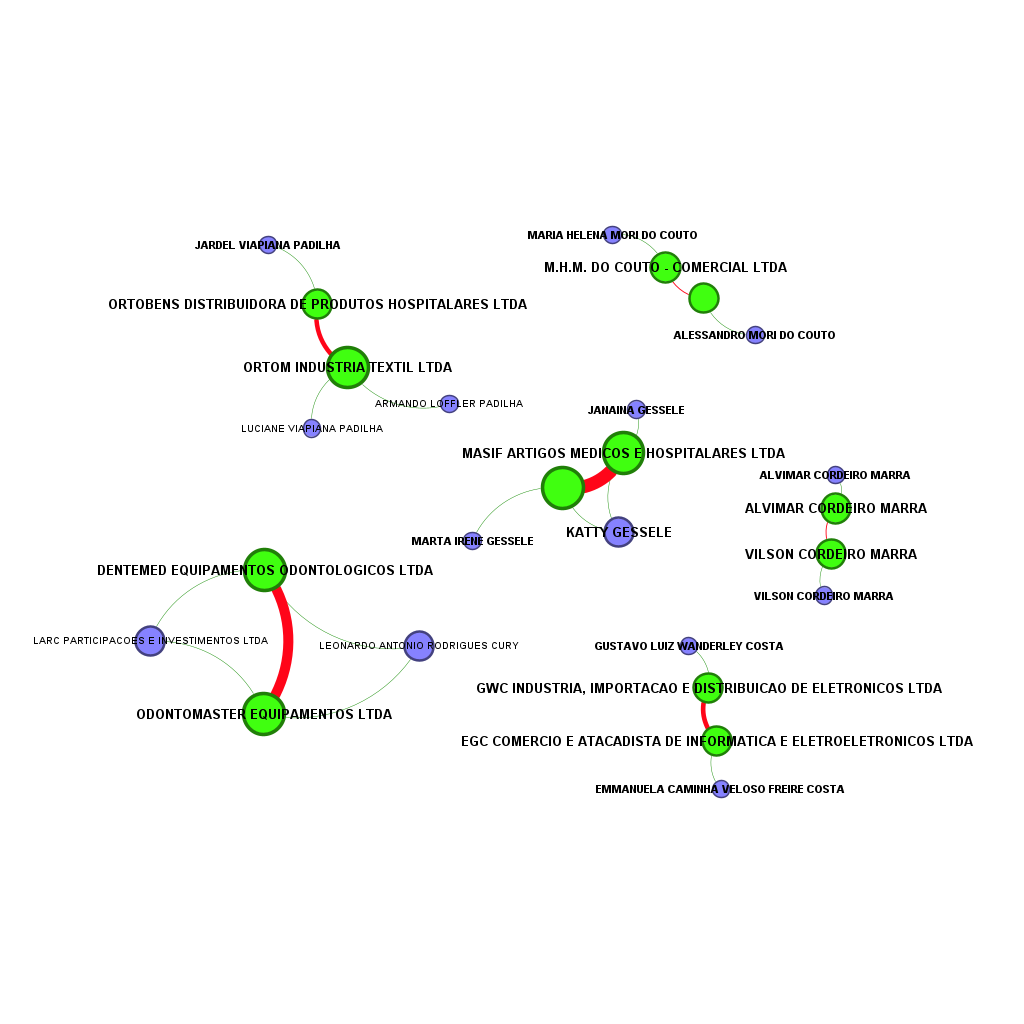
\includegraphics[width=\linewidth]{figures/Sub_grafo.png}
  \caption{Subgrafo de alto risco composto por seis componentes conexas independentes ($|V|=26$ e $|E|=23$). Os vértices representam empresas licitantes (verde) e sócios ou controladores (azul). As arestas verdes representam relações societárias, enquanto as vermelhas representam vínculos suspeitos, com espessura proporcional ao escore $s(a,b)$. Destacam-se os motivos triangulares $K_3$ nos Casos 1 e 2, associados ao compartilhamento de controladores entre empresas concorrentes.}
  \label{fig:subgrafo-alto-risco}
\end{figure}

A análise individualizada dos componentes permitiu identificar diferentes combinações de evidências cadastrais, societárias e onomásticas. A Tabela~\ref{tab:analise_nucleos} apresenta a decomposição dos escores atribuídos aos seis pares concorrentes, bem como os respectivos padrões topológicos e contextos licitatórios.

\begin{table*}[!t]
  \centering
  \caption{Caracterização dos Núcleos de Alto Risco Identificados}
  \label{tab:analise_nucleos}
  \footnotesize
  \begin{tabular}{clccp{8.0cm}}
    \hline
    \textbf{Caso} & \textbf{Par Concorrente} & \textbf{Escore} & \textbf{Motivo} & \textbf{Evidências Identificadas} \\
    \hline
    1 & \texttt{E1-A} $\times$ \texttt{E1-B} & 29,00 & $K_3$ & Uma sócia em comum ($+10{,}00$), endereço compartilhado em Curitiba/PR ($+10{,}00$), mesmo telefone com DDD 41 ($+8{,}00$) e um sobrenome raro ($+1{,}00$). Processo 36/2025, referente a materiais médico-cirúrgicos. \\
    2 & \texttt{E2-A} $\times$ \texttt{E2-B} & 22,25 & $2 \times K_3$ & Dois sócios em comum, sendo uma pessoa física e uma holding ($+20{,}00$), dois tokens raros ($+2{,}00$) e um sobrenome comum ($+0{,}25$). Concorrência em 59 itens do Processo 208/2025, referente a materiais odontológicos. \\
    3 & \texttt{E3-A} $\times$ \texttt{E3-B} & 10,25 & Árvore & Endereço normalizado compartilhado em Bayeux/PB ($+10{,}00$) e um sobrenome comum entre os sócios ($+0{,}25$). Recorrência de concorrência em certames de informática e eletrônicos. \\
    4 & \texttt{E4-A} $\times$ \texttt{E4-B} & 10,00 & Árvore & Telefone fixo compartilhado com DDD 15 ($+8{,}00$) e dois sobrenomes raros compartilhados entre os sócios ($+2{,}00$). Processo 48/2025, referente a materiais médicos descartáveis. \\
    5 & \texttt{E5-A} $\times$ \texttt{E5-B} & 2,00 & Árvore & Dois sobrenomes raros compartilhados entre titulares de MEI ($+2{,}00$). Processo 61/2025, referente a transporte escolar. \\
    6 & \texttt{E6-A} $\times$ \texttt{E6-B} & 2,00 & Árvore & Dois sobrenomes raros compartilhados entre sócios ($+2{,}00$). Processo 111/2025, referente a equipamentos hospitalares. \\
    \hline
  \end{tabular}
\end{table*}

A distribuição dos escores evidencia diferentes níveis de sobreposição entre os pares analisados. Os Casos 1 e 2 apresentam as maiores pontuações, associadas à existência de sócios compartilhados e, consequentemente, à formação de motivos triangulares na rede. Nos demais casos, os vínculos identificados decorrem principalmente de coincidências domiciliares, telefônicas ou onomásticas, sem compartilhamento
formal de sócios identificado no QSA.

\subsubsection{Motivos Topológicos de Controle Societário Compartilhado}

A enumeração identificou três motivos estruturais $K_3$, concentrados nos Casos 1 e 2, conforme ilustrado na Fig.~\ref{fig:subgrafo-alto-risco}. Cada motivo é formado por um sócio compartilhado, duas empresas e três arestas: duas relações de propriedade entre o sócio e as empresas e uma relação \texttt{Vinculo\_Suspeito} entre as empresas. Formalmente, para um sócio $S_i$ compartilhado pelas empresas $E_a$ e $E_b$, o triângulo é dado por:

\begin{equation}
  \{(S_i,E_a),(S_i,E_b),(E_a,E_b)\},
  \label{eq:motivo_k3}
\end{equation}

em que as duas primeiras arestas pertencem à camada \texttt{É\_Dono\_De} e a terceira à camada \texttt{Vinculo\_Suspeito}. Portanto, o motivo triangular ocorre na representação agregada multicamada, e não na camada bipartida de propriedade considerada isoladamente.

O Caso 2 apresenta uma configuração de maior complexidade: as empresas \texttt{E2-A} e \texttt{E2-B} compartilham simultaneamente um sócio pessoa física (\texttt{S2-PF}) e uma holding controladora (\texttt{S2-Holding}), resultando em dois motivos triangulares ($2 \times K_3$). O registro descritivo informa disputa em 59 itens do Processo Licitatório nº 208/2025, enquanto o atributo \texttt{Peso\_Concorrencia} apresenta valor 60. Como a documentação disponível não esclarece a diferença entre a contagem de itens e o peso armazenado, os dois valores são mantidos como registrados, sem presumir que representem a mesma unidade de contagem.

Essa configuração constitui um dos principais alertas identificados pelo modelo, uma vez que empresas formalmente distintas apresentam convergência em dois níveis de controle societário e participação simultânea em múltiplos itens do mesmo certame. Esse padrão justifica investigação complementar sobre a independência das propostas e a autonomia decisória dos concorrentes.

No Caso 1, o escore de 29{,}00 resulta da combinação de uma sócia compartilhada ($+10{,}00$), endereço coincidente em Curitiba/PR ($+10{,}00$), telefone compartilhado com DDD 41 ($+8{,}00$) e sobrenome raro em comum ($+1{,}00$). A convergência simultânea desses atributos indica forte sobreposição cadastral e societária entre as empresas concorrentes, constituindo outro núcleo prioritário para análise pericial.

\subsubsection{Indícios de Vínculos Operacionais e Onomásticos
sem Compartilhamento Societário Direto}

Os Casos 3 a 6 apresentam componentes conexas com estrutura em árvore, sem a formação de motivos triangulares $K_3$. Nesses casos, não foi identificado compartilhamento formal de sócios no QSA. Entretanto, a avaliação multidimensional permitiu detectar outras formas de
sobreposição entre os participantes, que seriam menos evidentes em análises restritas à interseção de CPF ou CNPJ dos quadros societários.

Nos Casos 3 e 4, predominam evidências relacionadas ao compartilhamento de infraestrutura cadastral e de contato. No Caso 3, as empresas \texttt{E3-A} e \texttt{E3-B} apresentam o mesmo endereço normalizado em Bayeux/PB, além de recorrência de concorrência em certames de informática e eletrônicos. Essa recorrência é registrada em \texttt{Peso\_Concorrencia} e não integra o escore $s(a,b)$. No Caso 4, as empresas \texttt{E4-A} e \texttt{E4-B} compartilham um terminal telefônico fixo com DDD 15 e apresentam dois sobrenomes raros em comum entre seus respectivos sócios. 

Nos Casos 5 e 6, os principais elementos de sobreposição são de natureza onomástica. A ponderação diferencial dos sobrenomes, com atribuição de peso 1{,}00 para sobrenomes classificados como raros, permitiu identificar dois sobrenomes compartilhados entre titulares de MEI no setor de transporte escolar (Caso 5) e entre sócios de empresas fornecedoras de equipamentos hospitalares (Caso 6).

Embora esses quatro componentes não apresentem compartilhamento societário formal identificado, as coincidências observadas constituem indicadores complementares para a análise das relações entre concorrentes. Sua interpretação, contudo, deve considerar a possibilidade de coincidências cadastrais, vínculos familiares ou outros fatores que não caracterizam, isoladamente, coordenação ilícita entre empresas.
